\documentclass[12pt,addpoints]{repaso}
\grado{4}
\nivel{Primaria}
\cicloescolar{2024-2025}
\materia{Matemáticas}
\unidad{3}
\title{Practica la Unidad}
\aprendizajes{\tiny
      \item Expresa oralmente la sucesión numérica hasta cuatro cifras, en español y hasta donde sea posible, en su lengua materna, de manera ascendente y descendente a partir de un número natural dado.
      \item Representa, con apoyo de material concreto y modelos gráficos, fracciones: medios, cuartos, octavos, dieciseisavos, para expresar el resultado de mediciones y repartos en situaciones vinculadas a su contexto.
      \item Resuelve situaciones problemáticas vinculadas a su contexto que implican sumas o restas de números naturales de hasta cuatro cifras utilizando los algoritmos convencionales y números decimales hasta centésimos, con apoyo de material concreto y representaciones gráficas.
	  \item Resuelve situaciones problemáticas que implican sumas o restas de fracciones con diferente denominador (tercios, quintos, sextos, novenos y décimos) vinculados a su contexto, mediante diversos procedimientos, en particular, la equivalencia.
	  \item Resuelve situaciones problemáticas vinculadas a su contexto que implican multiplicaciones de números naturales de hasta tres por dos cifras, a partir de diversas descomposiciones aditivas y el algoritmo convencional y el uso de un algoritmo para dividir números naturales de hasta tres cifras entre un número de una o dos cifras; reconoce al cociente y al residuo como resultado de una división.
	  }
\author{Melchor Pinto, JC}
\begin{document}
\INFO
\begin{questions}
	% UNIDAD 3                  
	% \section*{\ifprintanswers{Introducción a fracciones                  }\else{}\fi}
	% \subsection*{\ifprintanswers{Clasificación de fracciones                }\else{}\fi}

	\questionboxed[4]{Clasifica las siguientes fracciones en propias, impropias o mixtas:

		\begin{multicols}{3}
			\begin{parts}\Large
				\part $\dfrac{5}{6}$   \fillin[Propia][1in]   \\[1em]
				\part $5\dfrac{5}{11}$ \fillin[Mixta][1in]    \\[1em]
				\part $\dfrac{7}{3}$   \fillin[Impropia][1in] \\[1em]
				\part $\dfrac{3}{4}$   \fillin[Propia][1in]   \\[1em]
				\part $1\dfrac{2}{3}$  \fillin[Mixta][1in]    \\[1em]
				\part $\dfrac{7}{5}$   \fillin[Impropia][1in] \\[1em]
				\part $\dfrac{7}{8}$   \fillin[Propia][1in]   \\[1em]
				\part $3\dfrac{2}{9}$  \fillin[Mixta][1in]    \\[1em]
				\part $\dfrac{3}{2}$   \fillin[Impropia][1in] \\[1em]
				% \part $4\dfrac{1}{4}=$ \fillin[Mixta][1in]  
			\end{parts}
		\end{multicols}
	}

	% \subsection*{\ifprintanswers{Representación de fracciones}\else{}\fi}
	\questionboxed[2]{Escribe sobre la línea la fracción que representa cada imagen:

		\begin{multicols}{5}
			\begin{parts}
				\part 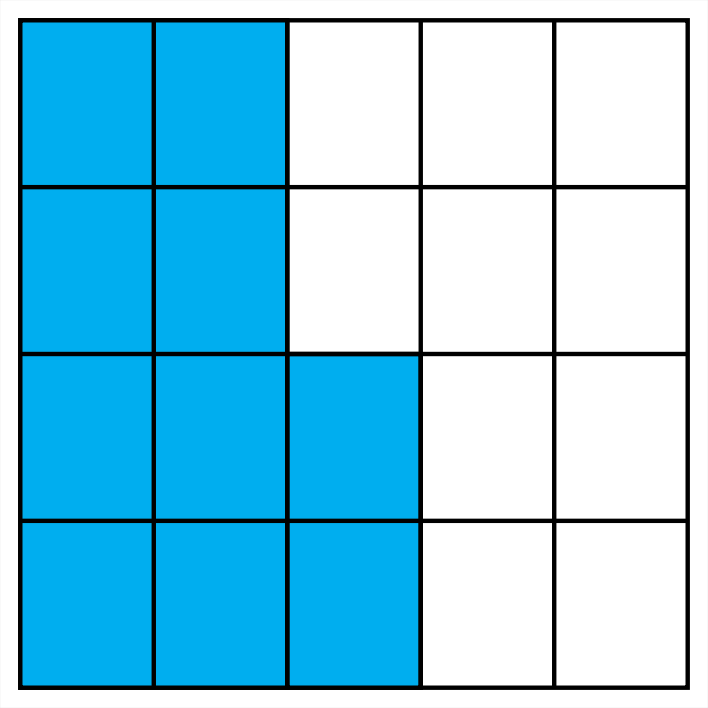
\includegraphics[width=45px]{../images/imagen_frac01.png} \fillin[\fbox{$\dfrac{10}{20}$}][0in] \\[1em]
				\part 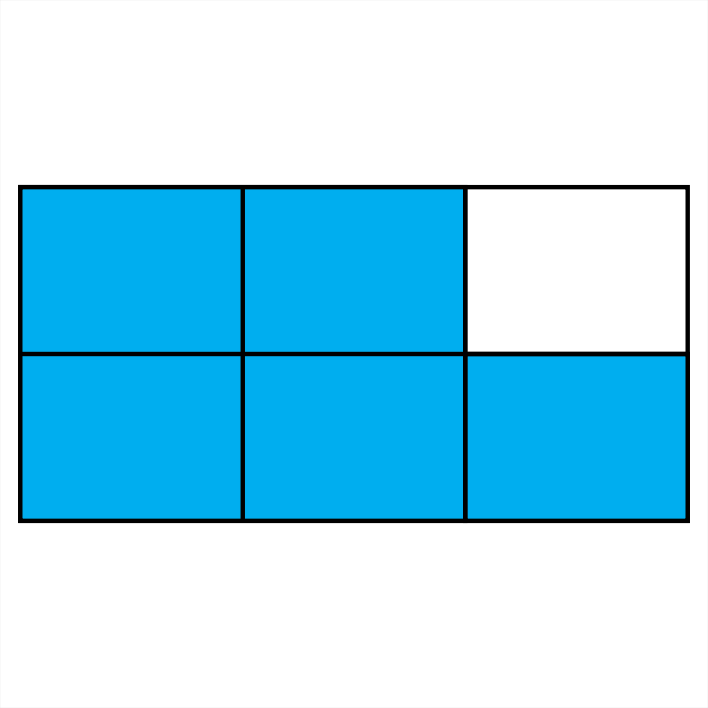
\includegraphics[width=45px]{../images/imagen_frac02.png} \fillin[\fbox{$\dfrac{5}{6}$}][0in] \\[1em]
				\part 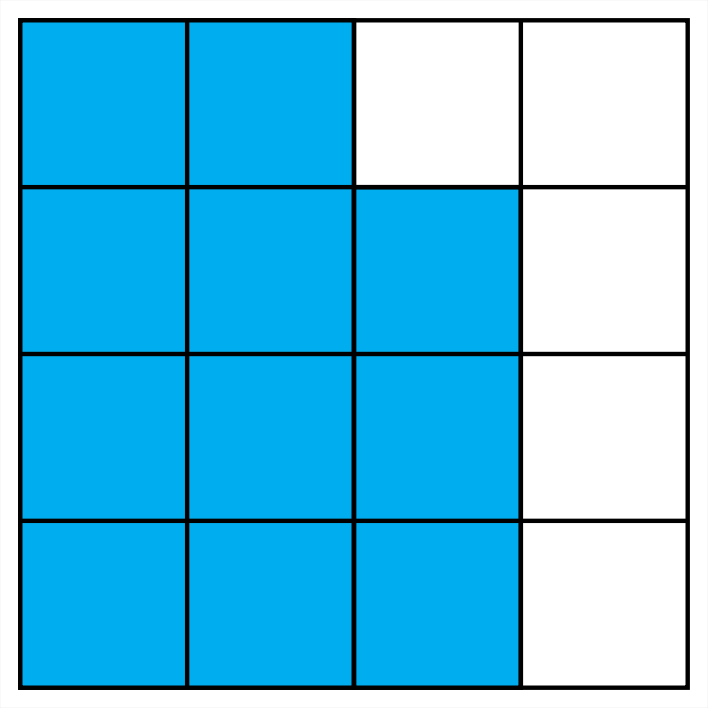
\includegraphics[width=45px]{../images/imagen_frac03.png} \fillin[\fbox{$\dfrac{11}{16}$}][0in] \\[1em]
				\part 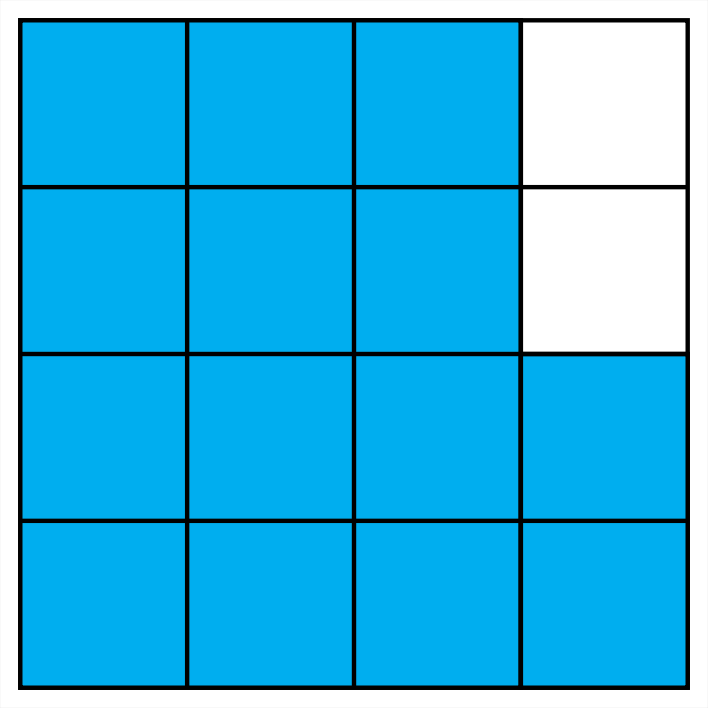
\includegraphics[width=45px]{../images/imagen_frac04.png} \fillin[\fbox{$\dfrac{14}{16}$}][0in] \\[1em]
				\part 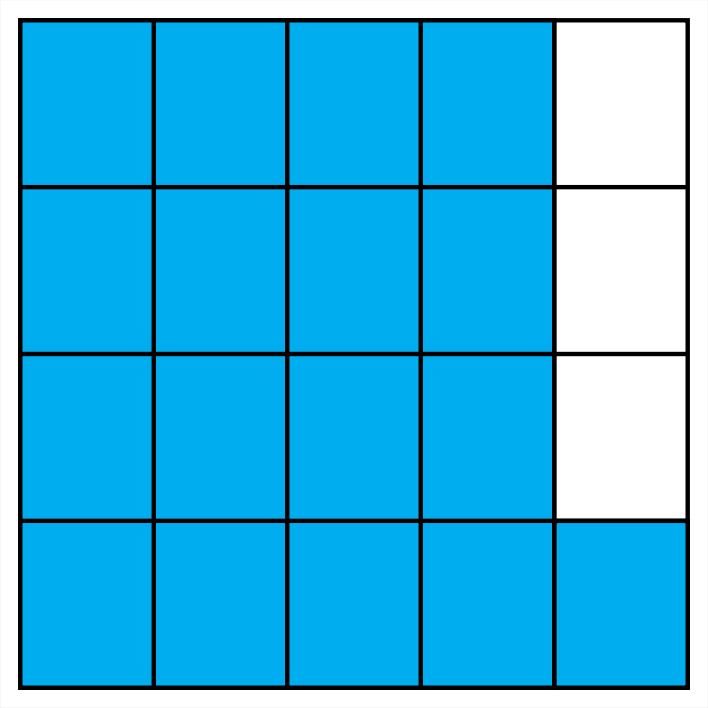
\includegraphics[width=45px]{../images/imagen_frac05.png} \fillin[\fbox{$\dfrac{17}{20}$}][0in] \\[1em]
				\part 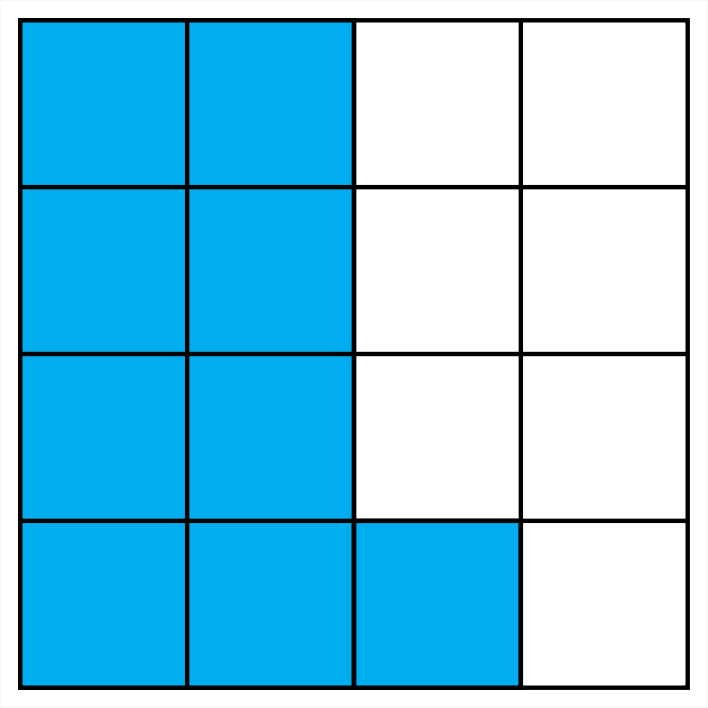
\includegraphics[width=45px]{../images/imagen_frac06.png} \fillin[\fbox{$\dfrac{9}{16}$}][0in] \\[1em]
				\part 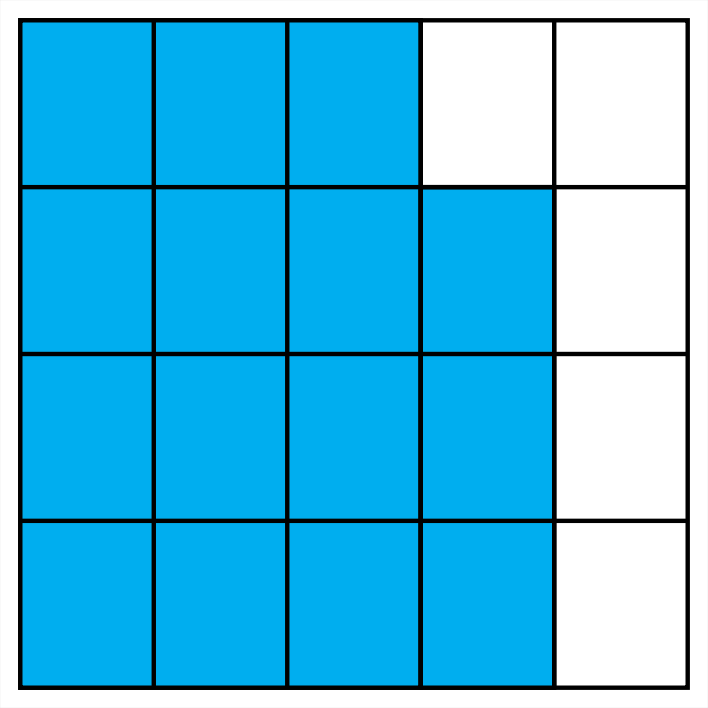
\includegraphics[width=45px]{../images/imagen_frac07.png} \fillin[\fbox{$\dfrac{15}{20}$}][0in] \\[1em]
				\part 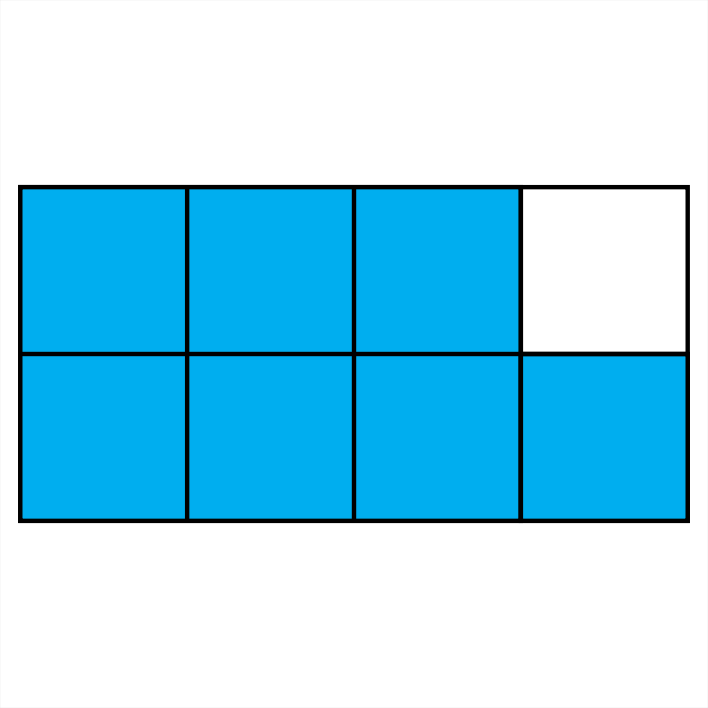
\includegraphics[width=45px]{../images/imagen_frac08.png} \fillin[\fbox{$\dfrac{7}{8}$}][0in] \\[1em]
				\part 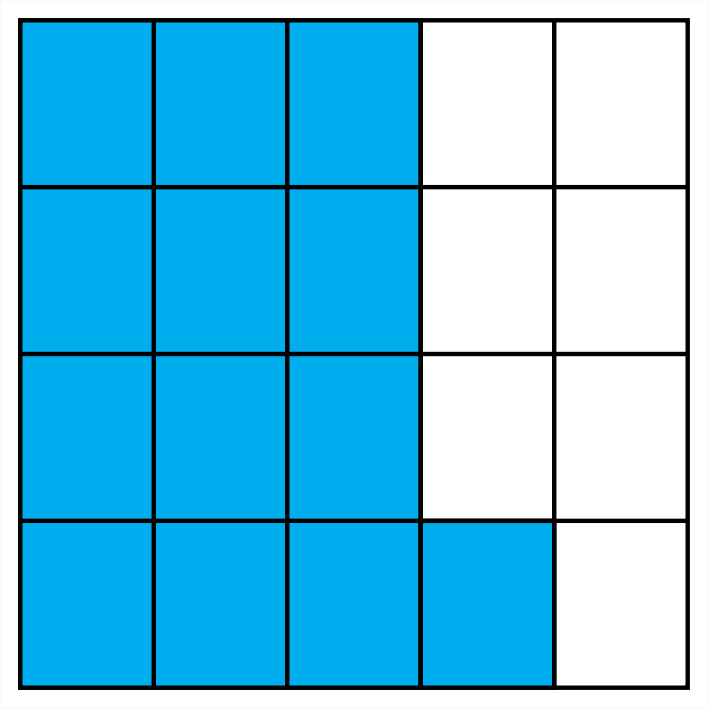
\includegraphics[width=45px]{../images/imagen_frac09.png} \fillin[\fbox{$\dfrac{13}{20}$}][0in] \\[1em]
				\part 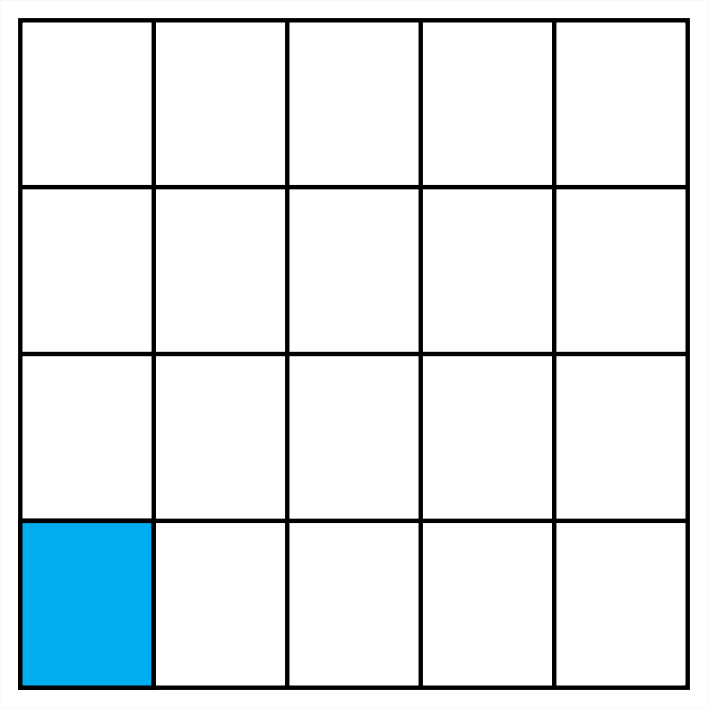
\includegraphics[width=45px]{../images/imagen_frac11.png} \fillin[\fbox{$\dfrac{1}{20}$}][0in] \\[1em]
			\end{parts}
		\end{multicols}
	}


	% \subsection*{\ifprintanswers{Nombre de fracciones                       }\else{}\fi}

	\questionboxed[2]{Escribe la fracción que corresponda en cada inciso:

		\begin{parts}
			\part ¿Cómo se escribe numéricamente la fracción \textbf{ocho quintos}?    \fillin[$\dfrac{8}{5}$][0in]  \\
			\part ¿Cómo se escribe numéricamente la fracción \textbf{seis onceavos}?   \fillin[$\dfrac{6}{11}$][0in] \\
			\part ¿Cómo se escribe numéricamente la fracción \textbf{dos séptimos}?    \fillin[$\dfrac{2}{7}$][0in]  \\
			\part ¿Cómo se escribe numéricamente la fracción \textbf{once medios}?     \fillin[$\dfrac{11}{2}$][0in] \\
			\part ¿Cómo se escribe numéricamente la fracción \textbf{diez décimos}?    \fillin[$\dfrac{10}{10}$][0in]\\
		\end{parts}
	}

	% \subsection*{\ifprintanswers{Conversión de fracciones mixtas a impropias}\else{}\fi}
	\questionboxed[4]{Convierte la siguientes fracciones mixtas a impropias:

		\begin{multicols}{3}
			\begin{parts}\large
				\part $4\dfrac{2}{3}= $ \fillin[$\dfrac{14}{3}$][0in]
				\part $2\dfrac{3}{10}= $ \fillin[$\dfrac{23}{10}$][0in]
				\part $5\dfrac{1}{5}= $ \fillin[$\dfrac{26}{5}$][0in]
			\end{parts}
		\end{multicols}
	}


	% \subsection*{\ifprintanswers{Conversión de fracciones impropias a mixtas}\else{}\fi}

	\questionboxed[4]{Convierte la siguientes fracciones impropias a mixtas:

		\begin{multicols}{3}
			\begin{parts}\large
				\part $\dfrac{13}{3}= $ \fillin[$4\dfrac{1}{3}$][0in]
				\part $\dfrac{63}{10}= $ \fillin[$6\dfrac{3}{10}$][0in]
				\part $\dfrac{51}{5}= $ \fillin[$10\dfrac{1}{5}$][0in]
			\end{parts}
		\end{multicols}
	}

	% \section*{\ifprintanswers{Operaciones con fracciones                 }\else{}\fi}
	% \subsection*{\ifprintanswers{Suma de fracciones                         }\else{}\fi}
	% \subsection*{\ifprintanswers{Resta de fracciones                        }\else{}\fi}
	% \subsection*{\ifprintanswers{Multiplicación de fracciones               }\else{}\fi}
	% \subsection*{\ifprintanswers{División de fracciones                     }\else{}\fi}
	% \subsection*{\ifprintanswers{Operaciones de fracciones mixtas           }\else{}\fi}

	\questionboxed[15]{Realiza las siguientes operaciones.

		\begin{multicols}{2}
			\begin{parts}\large
				\part $\dfrac{3}{10}+\dfrac{4}{5}=$ \fillin[$\dfrac{11}{10} = 1\dfrac{1}{10}$][0in] \\[0.75em]
				\part $\dfrac{3}{4}-\dfrac{2}{5}=$ \fillin[$\dfrac{7}{20}$][0in] \\[0.75em]
				\part $\dfrac{2}{3}-\dfrac{2}{5}=$ \fillin[$\dfrac{4}{15}$][0in] \\[0.75em]
				\part $\dfrac{3}{8}+\dfrac{7}{10}=$ \fillin[$\dfrac{43}{40} = 1\dfrac{3}{40}$][0in] \\[0.75em]
				\part $\dfrac{3}{5}\times\dfrac{2}{3}=$ \fillin[$\dfrac{6}{15}$][0in]   \\[0.75em]
				\part $\dfrac{7}{8}\times\dfrac{3}{4}=$ \fillin[$\dfrac{21}{32}$][0in] \\[0.75em]
				\part $\dfrac{3}{5} \divisionsymbol\dfrac{2}{3}=$ \fillin[$\dfrac{9}{10}$][0in] \\[0.75em]
				\part $\dfrac{7}{8} \divisionsymbol\dfrac{3}{4}=$ \fillin[$\dfrac{28}{24}$][0in]	\\[0.75em]
			\end{parts}
		\end{multicols}
	}

	% \section*{\ifprintanswers{Figuras geométricas                        }\else{}\fi}
	% \subsection*{\ifprintanswers{Nombre de figuras                          }\else{}\fi}
	% \subsection*{\ifprintanswers{Elementos de figuras                       }\else{}\fi}

	\questionboxed[2]{Escribe sobre la línea el nombre que recibe cada figura geométrica de acuerdo con su número de lados:

		\begin{multicols}{3}
			\begin{parts}
				\part 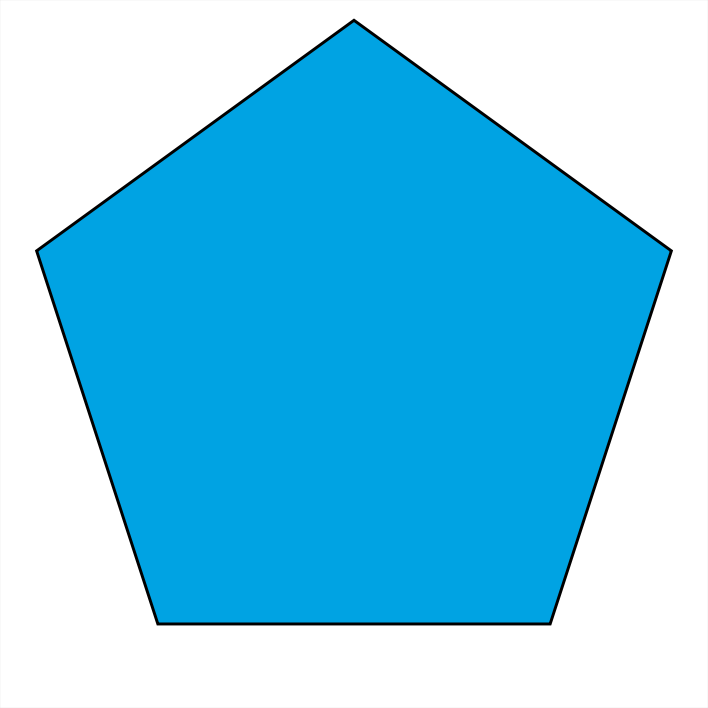
\includegraphics[width=75px]{../images/pentagono_azul.png}  \fillin[pentágono][0.75in]
				\part 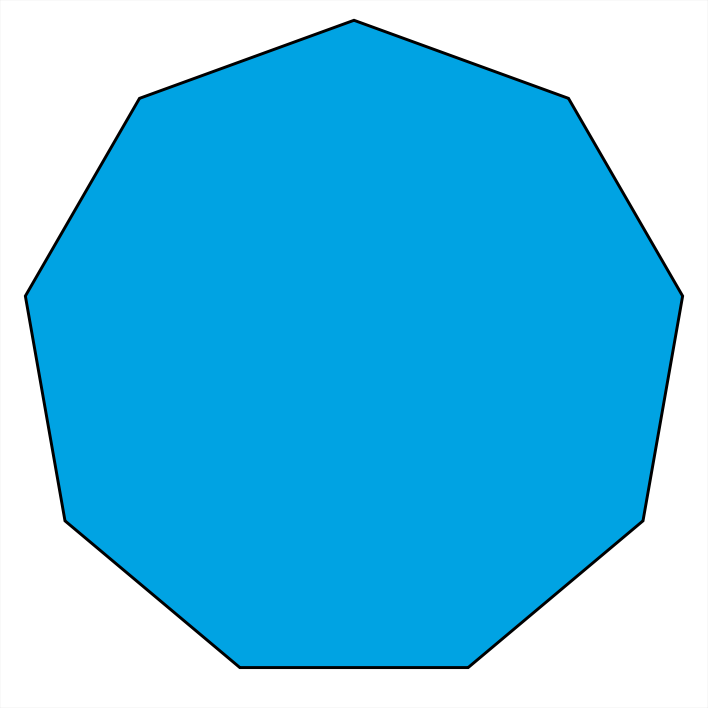
\includegraphics[width=75px]{../images/nonagono_azul.png}   \fillin[nonágono][0.75in]
				\part 
\includegraphics[width=75px]{../images/decagono_azul.png}   \fillin[decágono][0.75in]
				\part 
\includegraphics[width=75px]{../images/hexagono_azul.png}   \fillin[hexágono][0.75in]
				\part 
\includegraphics[width=75px]{../images/rectangulo_azul.png} \fillin[rectángulo][0.75in]
				\part 
\includegraphics[width=75px]{../images/cuadrado_azul.png}   \fillin[cuadrado][0.75in]
			\end{parts}
		\end{multicols}
	}


	% \subsection*{\ifprintanswers{Perímetros 1                               }\else{}\fi}
	% \subsection*{\ifprintanswers{Perímetros 2                               }\else{}\fi}

	\questionboxed[4]{Contesta las preguntas sobre perímetros de figuras geométricas

		\begin{multicols}{2}
			\begin{parts}\large
				% \part ¿Cuál es el perímetro de un rectángulo cuya base mide 15 y su altura mide 6?

				% \begin{solutionbox}{1cm}
				% 	\[P=15+6+15+6=\color{red}42\]
				% \end{solutionbox}

				\part ¿Cuál es el perímetro de un rectángulo cuya base mide 38 y su altura mide 19?

				\begin{solutionbox}{1cm}
					\[P=38+19+38+19=\color{red}114\]
				\end{solutionbox}

				\part ¿Cuál es el perímetro de un cuadrado que sus lados miden 5?

				\begin{solutionbox}{1cm}
					\[P=5+5+5+5=\color{red}20\]
				\end{solutionbox}

				\part ¿Cuál es el perímetro de un pentágono que sus lados miden 18?

				\begin{solutionbox}{1cm}
					\[P=18 \times 5=\color{red}90\]
				\end{solutionbox}

				% \part ¿Cuál es el perímetro de un octágono que sus lados miden 15?

				% \begin{solutionbox}{1cm}
				% 	\[P=15 \times 8=\color{red}120\]
				% \end{solutionbox}

				\part ¿Cuál es el perímetro de un rombo que sus lados miden 16?

				\begin{solutionbox}{1cm}
					\[P=16 \times 4=\color{red}64\]
				\end{solutionbox}

			\end{parts}
		\end{multicols}
	}

	% \subsection*{\ifprintanswers{Área de figuras                            }\else{}\fi}

	\questionboxed[4]{Contesta las preguntas sobre áreas de figuras geométricas

		\begin{multicols}{2}
			\begin{parts}\large
				\part ¿Cuál es el área de un triángulo cuya base mide 18 y su altura mide 11?

				\begin{solutionbox}{1.5cm}
					\[P=\dfrac{18 \times 11}{2}=\color{red}99\]
				\end{solutionbox}

				\part ¿Cuál es el área de un cuadrado que sus lados miden 29?

				\begin{solutionbox}{1.5cm}
					\[P=29 \times 29=\color{red}841\]
				\end{solutionbox}
			\end{parts}
		\end{multicols}
	}
	% \section*{\ifprintanswers{Sistema de unidades                        }\else{}\fi}
	% \subsection*{\ifprintanswers{Reloj                                      }\else{}\fi}
	% \subsection*{\ifprintanswers{Multiplicaciones por múltiplos de 10       }\else{}\fi}

	\questionboxed[3]{Realiza las siguientes operaciones:

		\begin{multicols}{3}
			\begin{parts}\large
				\part $ 55 \times 10000=$   \fillin[550000][0.5in]
				\part $ 135 \times 100=$   \fillin[13500][0.5in]
				\part $ 369 \times 10000=$   \fillin[3690000][0.5in]
				\part $ 88 \times 10=$   \fillin[880][0.5in]
				\part $ 1215 \times 100=$   \fillin[121500][0.5in]
				\part $ 300 \times 10000=$   \fillin[3000000][0.5in]
				\part $ 224 \times 1000=$   \fillin[224000][0.5in]
				\part $ 13 \times 1000=$   \fillin[13000][0.5in]
				\part $ 134 \times 100000=$   \fillin[13400000][0.5in]
				\part $ 188 \times 10=$   \fillin[1880][0.5in]
				\part $ 401 \times 1000=$   \fillin[401000][0.5in]
				\part $ 42 \times 10=$   \fillin[420][0.5in]
				\part $ 92 \times 1000=$   \fillin[92000][0.5in]
				\part $ 1050 \times 1000=$   \fillin[1050000][0.5in]
				\part $ 19 \times 100=$   \fillin[1900][0.5in]
			\end{parts}
		\end{multicols}
	}



	% \subsection*{\ifprintanswers{Unidades de tiempo                         }\else{}\fi}
	% \subsection*{\ifprintanswers{Unidades de longitud                       }\else{}\fi}

	\questionboxed[3]{Realiza las siguientes conversiones de unidades de longitud:

		\begin{multicols}{2}
			\begin{parts}
				\part De 157 kilómetros a hectómetros. \hfill \fillin[1570][0.6in] hm \\
				\part De 25 centímetros a milímetros.  \hfill \fillin[250][0.6in] mm \\
				\part De 27 kilómetros a decámetros.   \hfill \fillin[2700][0.6in] Dm \\
				\part De 17 kilómetros a hectómetros.  \hfill \fillin[170][0.6in] hm \\
				\part De 69 kilómetros a centímetros.  \hfill \fillin[6900000][0.6in] cm \\
				\part De 59 decímetros a centímetros.  \hfill \fillin[590][0.6in] cm \\
				\part De 26 metros a decímetros.       \hfill \fillin[260][0.6in] dm \\
				\part De 4 kilómetros a milímetros.    \hfill \fillin[4000000][0.6in] mm \\
				\part De 135 kilómetros a decámetros.  \hfill \fillin[13500][0.6in] Dm \\
				\part De 112 kilómetros a hectómetros. \hfill \fillin[1120][0.6in] hm \\
			\end{parts}
		\end{multicols}
	}


	% \subsection*{\ifprintanswers{Unidades de masa 	                          }\else{}\fi}
	\questionboxed[3]{Realiza las siguientes conversiones de unidades de longitud:

		\begin{multicols}{2}
			\begin{parts}\large
				\part De 205 gramos a decigramos    \hfill \fillin[2050][0.5in] dg \\
				\part De 25 kilogramos a gramos     \hfill \fillin[25000][0.5in] g \\
				\part De 58 kilogramos a gramos     \hfill \fillin[58000][0.5in] g \\
				\part De 45 decagramos a gramos     \hfill \fillin[450][0.5in] g \\
				\part De 134 gramos a decigramos    \hfill \fillin[1340][0.5in] dg \\
				\part De 282 gramos a miligramos    \hfill \fillin[282000][0.5in] mg \\
				\part De 117 decagramos a gramos    \hfill \fillin[1170][0.5in] g \\
				\part De 17 decigramos a miligramos \hfill \fillin[1700][0.5in] mg \\
				\part De 115 gramos a centigramos   \hfill \fillin[11500][0.5in] cg \\
				\part De 62 gramos a miligramos     \hfill \fillin[62000][0.5in] mg \\
			\end{parts}
		\end{multicols}
	}

\end{questions}
\end{document}